\newpage
\clearpage
\appendix
\textbf{\Large Appendix}

\addtocontents{toc}{\protect\setcounter{tocdepth}{2}}

\tableofcontents
\clearpage
\section{Experimental Details}
\label{appendix:setup}

\method evaluates memory mechanisms under realistic streaming multi-task conditions. In what follows, we describe the benchmark datasets, metrics, configurations and the methods compared in details.


\subsection{Datasets}
We evaluate our approach on a diverse suite of benchmarks that span factual knowledge, reasoning, mathematics, programming, and goal-oriented interaction.

We first introduce a suite of single-turn datasets designed to evaluate diverse reasoning abilities. \textbf{MMLU-Pro}~\citep{zheng2024mmlu} extends the original MMLU benchmark with stronger robustness and challenge by filtering data leakage, reducing ambiguity, and introducing more difficult questions across domains such as engineering, philosophy, and economics, making it a more reliable testbed for assessing multi-disciplinary reasoning. \textbf{GPQA-Diamond}~\citep{rein2023gpqa} is a graduate-level benchmark featuring expert-written, ``Google-proof'' questions in physics and related sciences, with its Diamond split being the most challenging and requiring rigorous multi-step reasoning. \textbf{AIME-24} and \textbf{AIME-25}~\citep{aime2024,aime2025} consist of Olympiad-style mathematics problems from the 2024 and 2025 American Invitational Mathematics Examinations, testing symbolic manipulation and problem-solving under strict exact-match criteria. Finally, \textbf{ToolBench}~\citep{patil2023gorilla} assesses a model’s ability to identify and configure external APIs, reflecting practical tool-use capabilities.


We then evaluate on a suite of multi-turn, goal-oriented benchmarks designed to evaluate memory in embodied and interactive environments. It includes several representative domains:
\textbf{AlfWorld}~\citep{shridhar2021alfworld} for household instruction following, 
\textbf{BabyAI}~\citep{chevalier2018babyai} for grounded navigation and compositional reasoning,
\textbf{ScienceWorld}~\citep{wang2022scienceworld} for open-ended scientific experimentation, 
\textbf{Jericho}~\citep{hausknecht2019interactive} for text-based game exploration, 
and \textbf{PDDL} tasks~\citep{yang2023pddlbench} for symbolic planning. 
Together, these environments emphasize long-horizon reasoning, sequential decision-making, and the use of accumulated experience to achieve complex goals.

Together, these datasets form a comprehensive benchmark suite that evaluates factual recall, domain expertise, mathematical reasoning, and procedural memory in interactive settings. This diversity enables a unified evaluation of both static and evolving capabilities, reflecting how LLMs learn, act, and adapt across academic and real-world scenarios.

\subsection{Configuration}

For efficient retrieval and fair comparison across methods, we utilize the BAAI/bge-base-en-v1.5~\citep{bge_m3} encoder as the retriever to index both queries and memory items.
During inference, the current question is encoded as a query and compared with all stored memory embeddings, retrieving the top-$k$ most relevant items (default $k=4$) for contextual augmentation.
This setting ensures a consistent retrieval budget across all methods.
For efficiency, retrieved texts and task inputs are truncated to fit within the same prompt length constraint used by the generation models.

While all baselines adopt the same retrieval configuration, certain methods (e.g., \textsc{Self-RAG}, \textsc{ReMem}) introduce additional reasoning modules that determine \emph{whether to retrieve} and \emph{what to retrieve} at each step. These adaptive behaviors operate on top of the same retrieval pool to ensure comparability.

Across all experiments, we maintain a unified task sequence ordering within each dataset, ensuring consistent memory evolution dynamics for all models. Unless otherwise specified, retrieval and generation operate within the same pipeline, and the retrieved items are appended to the prompt following the order of relevance, from most to least similar.

We benchmark a broad range of agents and memory architectures instantiated on two strong \textbf{LLM backbones}: the Gemini-2.5 series~\citep{comanici2025gemini} (\textsc{Flash}, \textsc{Flash-Lite}, and \textsc{Pro}) and the Claude family~\citep{anthropic_claude4_2025} (\textsc{3.5-Haiku} and \textsc{3.7-Sonnet}).

\subsection{Evaluation}

\method evaluates both task performance and memory quality along four key dimensions: \begin{itemize}[itemsep=-0.2em, topsep=-0.3em, leftmargin=*] \item \textbf{Answer accuracy.} Evaluates whether the LLM produces correct outputs across tasks, reflecting its ability to incorporate past experiences into inference. \item \textbf{Success rate.} Measures whether the LLM agent successfully completes task goals, indicating its overall effectiveness in interactive or goal-oriented settings. \item \textbf{Step efficiency.} Tracks the number of steps required to complete a goal, assessing whether memory usage enables concise and scalable reasoning. \item \textbf{Sequence robustness.} Examines whether the LLM maintains consistent knowledge and performance across varying task orders, reflecting its ability to stably reuse prior experiences. \end{itemize}





\subsection{Methods}

We benchmark \method with a wide spectrum of agent and memory architectures to study how different designs impact \emph{test-time memory evolution}. All methods are instantiated on two strong \textbf{LLM backbones}: Gemini-2.5~\citep{comanici2025gemini} and Claude-3.5/3.7~\citep{anthropic_claude4_2025}. Our comparisons isolate the impact of memory architecture and update strategy. Differences in backbone capability are not the focus of the study. We group the evaluated approaches into four major families:

\paragraph{Agent Pipelines without Persistent Memory.}
\textbf{ReAct}~\citep{yao2023react} serves as a representative reasoning–action pipeline, where memory is limited to the immediate context. It generates interleaved reasoning traces and tool calls but does not explicitly store or evolve information.  
\textbf{Amem} extends this pipeline with a lightweight agentic memory that caches recent observations and reflections. It provides a minimal form of experience reuse without dedicated search or update policies, forming a bridge between memory-free agents and adaptive memory systems.

\paragraph{Adaptive Agentic Memory Methods.}
This group focuses on adaptive retrieval and self-evolving memory. \textbf{SelfRAG}~\citep{asai2023self} integrates dynamic retrieval and reflection to adaptively ground reasoning in prior contexts.  
\textbf{MemOS}~\citep{Li2025MemOSAO}, \textbf{Mem0}~\citep{mem0}, and \textbf{LangMem}~\citep{langchain} implement structured, agent-level memory systems that support read, write, and update operations. Within our unified interface, retrieval corresponds to the \emph{search} stage and updates correspond to \emph{evolve}. These methods represent adaptive long-term agents capable of continual refinement.

\paragraph{Memory-Based Agents for Procedural Memory.}
\textbf{Dynamic Cheatsheet (DC)}~\citep{suzgun2025dynamic} and \textbf{Agent Workflow Memory (AWM)}~\citep{Wang2024AgentWM} emphasize the reuse of procedural knowledge, encoding “how-to” information rather than static facts.  
We evaluate two DC variants, \textbf{DC-RS} (retrieval-based) and \textbf{DC-Cu} (curated), to analyze how workflow induction and update mechanisms influence stability and transfer. These methods test the potential of procedural memory as reusable strategy repositories.

\paragraph{Proposed: Evolving Memory Framework.}
\textbf{ExpRecent} maintains condensed episodic traces of recent task trajectories, while our \textbf{ExpRAG} family integrates the principles of retrieval-augmented reasoning with explicit \emph{test-time evolution}. \textbf{ReMem} applies iterative reflection and synthesis to refine memory embeddings over time.  
Together, these methods instantiate \method's design philosophy, treating reasoning, acting, and memory refinement as interleaved processes that co-adapt during deployment, enabling continual self-improvement and more human-like adaptation.

\section{Experiments}

We provide more experiments in the following.
\subsection{Additional Experiments}
\label{app:exp}
We further validate our findings through extensive benchmarking across multiple model families (Gemini-2.5-Flash-Lite, Claude-3.5-Haiku) and diverse datasets, as shown in Tables~\ref{tab:multi_full} and~\ref{tab:single_full}.
The performance trends remain consistent across all settings.
On both multi-turn embodied reasoning tasks (AlfWorld, BabyAI, PDDL, ScienceWorld) and single-turn reasoning tasks (AIME-24/25, GPQA, MMLU-Pro, ToolBench), \alg consistently outperforms conventional baselines and adaptive retrieval methods across model backbones.
These results confirm that the advantages of evolving-memory architectures are model-agnostic, highlighting continual task-level reflection as a general mechanism for improving adaptability in problem-solving.



\begin{table*}[t!]
\centering
\scriptsize
\setlength{\tabcolsep}{4pt}
\renewcommand{\arraystretch}{1.2}
\scalebox{0.9}{
\begin{tabular}{l l cc cc cc cc cc}
\toprule
\multirow{2}{*}{\textbf{LLM Backbone}} & \multirow{2}{*}{\textbf{Method}} 
& \multicolumn{2}{c}{\textbf{AlfWorld}} 
& \multicolumn{2}{c}{\textbf{BabyAI}} 
& \multicolumn{2}{c}{\textbf{PDDL}} 
& \multicolumn{2}{c}{\textbf{ScienceWorld}} 
& \multicolumn{2}{c}{\textbf{Avg.}} \\
\cmidrule(lr){3-4}\cmidrule(lr){5-6}\cmidrule(lr){7-8}\cmidrule(lr){9-10}\cmidrule(lr){11-12}
 &  & S & P & S & P & S & P & S & P & S & P \\
\midrule
\multirow{15}{*}{Gemini 2.5 Flash}
 & Baseline & 0.12 & 0.34 & \textbf{0.61} & \textbf{0.71} & 0.12 & 0.20 & 0.24 & 0.59 & 0.27 & 0.46 \\
 & History & 0.28 & 0.60 & 0.52 & 0.64 & 0.08 & 0.15 & 0.31 & 0.71 & 0.30 & 0.53 \\
\cmidrule(lr){2-12}
 & ReAct & 0.24 & 0.56 & 0.48 & 0.63 & \textbf{0.22} & \textbf{0.33} & 0.34 & 0.71 & 0.32 & 0.56 \\
 & Amem & 0.25 & 0.59 & 0.53 & 0.64 & 0.10 & 0.16 & 0.36 & 0.74 & 0.31 & 0.53 \\
\cmidrule(lr){2-12}
 & SelfRAG & 0.25 & 0.59 & 0.52 & 0.65 & 0.08 & 0.16 & 0.34 & 0.74 & 0.30 & 0.54 \\
 & Mem0 & 0.27 & 0.61 & 0.54 & 0.66 & 0.10 & 0.19 & 0.32 & 0.70 & 0.31 & 0.54 \\
\cmidrule(lr){2-12}
 & DC-Cu & 0.25 & 0.59 & 0.53 & 0.64 & 0.08 & 0.17 & 0.29 & 0.71 & 0.29 & 0.53 \\
 & DC-RS & 0.27 & 0.60 & 0.53 & 0.66 & 0.07 & 0.15 & 0.33 & 0.73 & 0.30 & 0.54 \\
 & AWM & 0.26 & 0.59 & 0.52 & 0.64 & 0.08 & 0.16 & 0.33 & 0.73 & 0.30 & 0.53 \\
\cmidrule(lr){2-12}
 & ExpRecent & 0.37 & 0.65 & 0.53 & 0.64 & 0.13 & 0.22 & 0.53 & \textbf{0.83} & 0.39 & 0.59 \\
 & ExpRAG & 0.59 & 0.79 & 0.56 & 0.65 & 0.17 & 0.27 & 0.53 & 0.81 & 0.46 & 0.63 \\
 & \textbf{ReMem} & \textbf{0.66} & \textbf{0.81} & 0.53 & 0.61 & \textbf{0.22} & \textbf{0.33} & \textbf{0.58} & 0.81 & \textbf{0.50} & \textbf{0.64} \\
\midrule
\multirow{15}{*}{Gemini 2.5 Pro}
 & Baseline & 0.04 & 0.39 & 0.37 & 0.47 & 0.20 & 0.33 & 0.22 & 0.60 & 0.21 & 0.45 \\
 & History & 0.19 & 0.52 & 0.40 & 0.48 & 0.25 & 0.38 & 0.60 & 0.84 & 0.36 & 0.56 \\
\cmidrule(lr){2-12}
 & ReAct & 0.02 & 0.26 & 0.43 & 0.55 & 0.13 & 0.22 & 0.30 & 0.68 & 0.22 & 0.43 \\
 & Amem & 0.16 & 0.50 & 0.42 & 0.49 & 0.23 & 0.38 & 0.59 & 0.85 & 0.35 & 0.56 \\
\cmidrule(lr){2-12}
 & SelfRAG & 0.16 & 0.49 & 0.43 & 0.50 & 0.22 & 0.35 & 0.57 & 0.84 & 0.34 & 0.55 \\
 & Mem0 & 0.16 & 0.49 & 0.41 & 0.49 & 0.22 & 0.37 & 0.53 & 0.81 & 0.33 & 0.54 \\
\cmidrule(lr){2-12}
 & DC-Cu & 0.17 & 0.50 & 0.40 & 0.47 & 0.28 & 0.40 & 0.53 & 0.82 & 0.35 & 0.55 \\
 & DC-RS & 0.18 & 0.51 & 0.42 & 0.50 & 0.27 & 0.40 & 0.59 & 0.85 & 0.37 & 0.57 \\
 & AWM & 0.20 & 0.52 & 0.38 & 0.46 & 0.20 & 0.37 & 0.57 & 0.83 & 0.34 & 0.54 \\
\cmidrule(lr){2-12}
 & ExpRecent & 0.36 & 0.61 & 0.54 & \textbf{0.64} & \textbf{0.35} & \textbf{0.47} & \textbf{0.69} & \textbf{0.89} & 0.49 & 0.64 \\
 & ExpRAG & 0.38 & 0.64 & 0.46 & 0.53 & 0.28 & 0.43 & 0.61 & 0.84 & 0.43 & 0.61 \\
 & \textbf{ReMem} & \textbf{0.51} & \textbf{0.70} & \textbf{0.56} & \textbf{0.64} & 0.25 & 0.38 & 0.66 & 0.86 & \textbf{0.50} & \textbf{0.65} \\
\midrule
\multirow{15}{*}{Claude 3.7 Sonnet}
  & Baseline & 0.18 & 0.49 & 0.51 & 0.66 & 0.17 & 0.39 & 0.10 & 0.53 & 0.24 & 0.52 \\
 & History & 0.50 & 0.73 & 0.48 & 0.66 & 0.65 & 0.85 & 0.32 & 0.74 & 0.49 & 0.74 \\
\cmidrule(lr){2-12}
 & ReAct & 0.51 & 0.75 & 0.57 & 0.72 & 0.75 & 0.91 & 0.44 & 0.77 & 0.57 & 0.79 \\
 & Amem & 0.48 & 0.73 & 0.46 & 0.64 & 0.62 & 0.84 & 0.33 & 0.73 & 0.47 & 0.73 \\
\cmidrule(lr){2-12}
 & SelfRAG & 0.52 & 0.75 & 0.46 & 0.64 & 0.65 & 0.84 & 0.31 & 0.74 & 0.49 & 0.74 \\
 & Mem0 & 0.51 & 0.74 & 0.48 & 0.66 & 0.65 & 0.84 & 0.37 & 0.76 & 0.50 & 0.75 \\
\cmidrule(lr){2-12}
 & DC-Cu & 0.50 & 0.74 & 0.50 & 0.67 & 0.62 & 0.84 & 0.33 & 0.75 & 0.49 & 0.75 \\
 & DC-RS & 0.50 & 0.74 & 0.52 & 0.68 & 0.62 & 0.84 & 0.34 & 0.74 & 0.50 & 0.75 \\
 & AWM & 0.49 & 0.73 & 0.53 & 0.68 & 0.60 & 0.82 & 0.34 & 0.74 & 0.49 & 0.74 \\
\cmidrule(lr){2-12}
 & ExpRecent & 0.66 & 0.83 & 0.63 & 0.73 & 0.53 & 0.76 & 0.49 & 0.82 & 0.58 & 0.79 \\
 & ExpRAG & 0.74 & 0.89 & 0.62 & 0.72 & 0.72 & 0.89 & 0.46 & 0.76 & 0.63 & 0.82 \\
 & ReMem & \textbf{0.92} & \textbf{0.96} & \textbf{0.73} & \textbf{0.83} & \textbf{0.83} & \textbf{0.95} & \textbf{0.62} & \textbf{0.89} & \textbf{0.78} & \textbf{0.91} \\
\midrule
\multirow{15}{*}{Claude 3.5 Haiku}
 & Baseline & 0.11 & 0.33 & 0.38 & 0.52 & 0.15 & 0.32 & 0.08 & 0.37 & 0.18 & 0.39 \\
 & History & 0.28 & 0.58 & 0.38 & 0.57 & 0.18 & 0.38 & 0.12 & 0.49 & 0.24 & 0.51 \\
\cmidrule(lr){2-12}
 & ReAct & 0.24 & 0.58 & 0.35 & 0.52 & 0.32 & 0.53 & 0.16 & 0.55 & 0.27 & 0.55 \\
 & Amem & 0.24 & 0.55 & 0.37 & 0.58 & 0.17 & 0.35 & 0.12 & 0.45 & 0.23 & 0.48 \\
\cmidrule(lr){2-12}
 & SelfRAG & 0.26 & 0.58 & 0.38 & 0.59 & 0.22 & 0.37 & 0.14 & 0.49 & 0.25 & 0.51 \\
 & Mem0 & 0.27 & 0.56 & 0.37 & 0.57 & 0.17 & 0.37 & 0.08 & 0.45 & 0.22 & 0.49 \\
\cmidrule(lr){2-12}
 & DC-Cu & 0.24 & 0.55 & 0.37 & 0.58 & 0.17 & 0.37 & 0.12 & 0.45 & 0.23 & 0.49 \\
 & DC-RS & 0.24 & 0.55 & 0.37 & 0.58 & 0.17 & 0.37 & 0.12 & 0.45 & 0.23 & 0.49 \\
 & AWM & 0.24 & 0.55 & 0.37 & 0.58 & 0.17 & 0.37 & 0.12 & 0.45 & 0.23 & 0.49 \\
\cmidrule(lr){2-12}
 & ExpRecent & 0.48 & 0.65 & 0.40 & 0.57 & 0.15 & 0.32 & 0.32 & 0.64 & 0.34 & 0.55 \\
 & ExpRAG & 0.65 & 0.74 & 0.54 & 0.64 & \textbf{0.43} & \textbf{0.61} & 0.42 & 0.68 & 0.51 & 0.67 \\
 & \textbf{ReMem} & \textbf{0.69} & \textbf{0.80} & \textbf{0.49} & \textbf{0.60} & \textbf{0.43} & \textbf{0.61} & \textbf{0.44} & \textbf{0.75} & \textbf{0.51} & \textbf{0.69} \\
\bottomrule
\end{tabular}}
\caption{Cross-environment results across four embodied reasoning benchmarks (AlfWorld, BabyAI, PDDL, ScienceWorld). Each dataset reports success (S) and progress (P) rates. Bold indicates the best (including ties) per column. The last two columns show averaged S and P across datasets.}
\label{tab:multi_full}
\end{table*}


\begin{table*}[t!]
\centering
\scriptsize
\setlength{\tabcolsep}{3.5pt}
\renewcommand{\arraystretch}{1.1}
\scalebox{0.85}{
\begin{tabular}{l l*{8}{c}}
\toprule
\multirow{2}{*}{\textbf{LLM Backbone}} & \multirow{2}{*}{\textbf{Method}} & \multicolumn{6}{c}{\textbf{Exact Match $\uparrow$}} & \multicolumn{1}{c}{\textbf{API / Acc. $\uparrow$}}\\
\cmidrule(lr){3-8}\cmidrule(lr){9-9}
 &  & AIME24 & AIME25 & GPQA & MMLU-Pro (Eco.) & MMLU-Pro (Eng.) & MMLU-Pro (Philo.) & ToolBench& \multicolumn{1}{c}{\textbf{Avg. $\uparrow$}}\\
\midrule

% ---------------- Claude 3.5 ----------------
\multirow{15}{*}{Claude 3.5}
 & Baseline   & \textemdash{} & \textemdash{} & 0.36 & 0.68 & 0.42 & 0.55 & 0.81/0.64 & 0.38 \\
 & History    & \textemdash{} & \textemdash{} & 0.37 & 0.70 & 0.43 & 0.55 & 0.81/0.63 & 0.38 \\
\cmidrule(lr){2-10}
 & ReAct      & \textemdash{} & \textemdash{} & 0.35 & 0.69 & 0.43 & 0.54 & 0.81/0.64 & 0.38 \\
 & Amem       & \textemdash{} & \textemdash{} & 0.34 & 0.69 & 0.43 & 0.53 & 0.82/0.63 & 0.37 \\
\cmidrule(lr){2-10}
 & SelfRAG    & \textemdash{} & \textemdash{} & 0.36 & 0.70 & 0.44 & 0.56 & 0.83/0.65 & 0.39 \\
 & MemOS      & \textemdash{} & \textemdash{} & 0.37 & 0.70 & 0.42 & 0.55 & 0.81/0.64 & 0.38 \\
 & Mem0       & \textemdash{} & \textemdash{} & 0.36 & 0.70 & 0.42 & 0.55 & 0.82/0.64 & 0.38 \\
 & LangMem    & \textemdash{} & \textemdash{} & \textbf{0.51} & \textbf{0.78} & 0.46 & 0.61 & 0.81/0.63 & \textbf{0.43} \\
\cmidrule(lr){2-10}
 & DC-RS      & \textemdash{} & \textemdash{} & 0.36 & 0.68 & 0.41 & 0.56 & 0.82/0.64 & 0.38 \\
 & AWM        & \textemdash{} & \textemdash{} & 0.33 & 0.67 & 0.42 & 0.53 & 0.81/0.63 & 0.37 \\
 & DC-Cu      & \textemdash{} & \textemdash{} & 0.33 & 0.65 & 0.39 & 0.54 & 0.82/0.63 & 0.36 \\
\cmidrule(lr){2-10}
 & ExpRecent  & \textemdash{} & \textemdash{} & 0.42 & 0.69 & 0.46 & 0.59 & 0.85/0.63 & 0.40 \\
 & ExpRAG     & \textemdash{} & \textemdash{} & 0.40 & 0.73 & \textbf{0.49} & 0.61 & 0.87/0.67 & 0.41 \\
 & ReMem      & \textemdash{} & \textemdash{} & 0.39 & 0.71 & 0.47 & \textbf{0.62} & \textbf{0.87/0.68} & 0.41 \\
\midrule

% ---------------- Claude 3.7 ----------------
\multirow{15}{*}{Claude 3.7 Sonnet}
 & Baseline            & 0.17 & 0.13 & 0.55 & 0.84 & 0.63 & 0.78 & 0.76/0.62 & 0.54 \\
 & History       & 0.13 & \textbf{0.23} & 0.56 & 0.85 & 0.64 & 0.78 & 0.76/0.61 & 0.55 \\
\cmidrule(lr){2-10}
 & ReAct                     & 0.17 & 0.10 & 0.57 & 0.84 & 0.63 & 0.76 & 0.76/0.61 & 0.54 \\
 & Amem                      & \textbf{0.27} & 0.17 & 0.54 & 0.83 & 0.63 & 0.79 & 0.77/0.63 & 0.56 \\
\cmidrule(lr){2-10}
 & SelfRAG                   & 0.20 & 0.10 & 0.58 & 0.84 & 0.65 & 0.77 & 0.77/0.63 & 0.55 \\
 & MemOS                     & 0.17 & 0.20 & 0.55 & 0.84 & 0.64 & 0.76 & 0.76/0.62 & 0.55 \\
 & Mem0                      & 0.20 & 0.13 & 0.58 & 0.84 & 0.62 & 0.77 & 0.76/0.61 & 0.55 \\
 & LangMem                   & 0.10 & 0.13 & 0.53 & 0.77 & 0.56 & 0.66 & 0.77/0.63 & 0.49 \\
\cmidrule(lr){2-10}
 & DC-RS                     & 0.20 & 0.20 & 0.62 & 0.79 & 0.52 & 0.60 & 0.77/0.62 & 0.52 \\
 & AWM                       & 0.03 & 0.03 & 0.53 & 0.80 & 0.56 & 0.72 & 0.76/0.62 & 0.48 \\
 & DC-Cu                     & 0.17 & \textbf{0.23} & 0.57 & 0.79 & 0.52 & 0.65 & 0.77/0.62 & 0.52 \\
\cmidrule(lr){2-10}
 & ExpRecent                 & 0.13 & 0.20 & 0.61 & \textbf{0.86} & 0.63 & 0.78 & 0.82/0.66 & 0.56 \\
 & ExpRAG                    & 0.17 & 0.17 & \textbf{0.70} & 0.85 & \textbf{0.67} & \textbf{0.80} & \textbf{0.88/0.72} & \textbf{0.59} \\
 & ReMem                     & 0.13 & 0.13 & 0.67 & \textbf{0.86} & 0.65 & 0.80 & 0.87/0.71 & 0.58 \\
\midrule


% ---------------- Gemini 2.5 Flash ----------------
\multirow{15}{*}{Gemini 2.5 Flash}
 & Baseline           & 0.47 & 0.47 & 0.48 & 0.83 & \textbf{0.46} & 0.75 & 0.71/0.61 & 0.59 \\
 & History       & 0.60 & 0.47 & 0.43 & 0.84 & 0.42 & 0.78 & 0.31/0.26 & 0.55 \\
\cmidrule(lr){2-10}
 & ReAct                    & 0.30 & 0.27 & 0.05 & 0.64 & 0.16 & 0.54 & 0.64/0.57 & 0.37 \\
 & Amem                     & \textbf{0.70} & \textbf{0.57} & 0.52 & 0.83 & 0.42 & 0.72 & 0.72/0.60 & 0.63 \\
\cmidrule(lr){2-10}
 & SelfRAG                  & 0.50 & 0.47 & 0.46 & 0.83 & 0.45 & 0.75 & 0.72/0.61 & 0.59 \\
 & MemOS                    & 0.47 & 0.47 & 0.50 & 0.82 & \textbf{0.46} & 0.75 & 0.71/0.61 & 0.59 \\
 & Mem0                     & 0.50 & 0.47 & 0.45 & 0.83 & \textbf{0.46} & 0.74 & 0.71/0.61 & 0.59 \\
 & LangMem                  & 0.43 & 0.50 & \textbf{0.53} & 0.79 & 0.39 & 0.71 & 0.68/0.57 & 0.57 \\
\cmidrule(lr){2-10}
 & DC-RS                    & 0.53 & 0.37 & 0.48 & 0.80 & 0.42 & 0.69 & 0.68/0.57 & 0.56 \\
 & DC-Cu                    & 0.60 & 0.40 & 0.48 & 0.79 & 0.44 & 0.69 & 0.70/0.59 & 0.58 \\
 & AWM                      & 0.50 & 0.37 & 0.49 & 0.79 & 0.43 & 0.72 & 0.71/0.59 & 0.56 \\
\cmidrule(lr){2-10}
 & ExpRecent                & 0.47 & 0.47 & 0.42 & 0.83 & 0.39 & 0.75 & 0.78/0.66 & 0.58 \\
 & ExpRAG                   & 0.43 & 0.47 & 0.42 & 0.83 & 0.43 & 0.78 & \textbf{0.87/0.73} & 0.60 \\
 & ReMem                    & 0.60 & 0.53 & 0.51 & \textbf{0.85} & \textbf{0.46} & \textbf{0.79} & 0.85/0.71 & \textbf{0.65} \\
\midrule


% ---------------- Gemini 2.5 Flash-Lite ----------------
\multirow{15}{*}{Gemini 2.5 Flash-Lite}
 & Baseline          & 0.53 & \textbf{0.43} & 0.37 & 0.73 & 0.34 & 0.60 & 0.78/0.61 & 0.58 \\
 & History     & 0.40 & 0.33 & 0.31 & 0.74 & 0.30 & 0.59 & 0.58/0.47 & 0.49 \\
\cmidrule(lr){2-10}
 & ReAct                   & 0.53 & 0.33 & 0.34 & 0.61 & 0.20 & 0.48 & 0.73/0.56 & 0.50 \\
 & Amem                    & 0.40 & 0.33 & 0.33 & 0.72 & \textbf{0.34} & 0.59 & 0.77/0.61 & 0.54 \\
\cmidrule(lr){2-10}
 & SelfRAG                 & \textbf{0.57} & 0.37 & 0.37 & 0.73 & 0.32 & 0.62 & 0.81/0.63 & 0.57 \\
 & MemOS                   & 0.53 & \textbf{0.43} & 0.37 & 0.73 & 0.34 & 0.60 & 0.78/0.61 & 0.58 \\
 & Mem0                    & 0.53 & \textbf{0.43} & 0.37 & 0.73 & 0.34 & 0.60 & 0.78/0.61 & 0.58 \\
 & LangMem                 & 0.40 & 0.37 & \textbf{0.48} & 0.59 & 0.24 & 0.56 & 0.33/0.26 & 0.43 \\
\cmidrule(lr){2-10}
 & DC-RS                   & 0.53 & \textbf{0.43} & 0.34 & 0.59 & 0.18 & 0.36 & 0.73/0.56 & 0.49 \\
 & AWM                     & 0.03 & 0.03 & 0.35 & 0.61 & 0.20 & 0.48 & 0.77/0.60 & 0.44 \\
 & DC-Cu                   & 0.53 & \textbf{0.43} & 0.33 & 0.55 & 0.16 & 0.32 & 0.71/0.56 & 0.47 \\
\cmidrule(lr){2-10}
 & ExpRecent               & \textbf{0.57} & 0.33 & 0.35 & 0.76 & 0.29 & 0.62 & 0.82/0.65 & 0.58 \\
 & ExpRAG                  & 0.47 & 0.37 & 0.38 & \textbf{0.79} & 0.32 & \textbf{0.66} & \textbf{0.87/0.68} & \textbf{0.61} \\
 & ReMem                   & \textbf{0.57} & 0.33 & 0.38 & 0.77 & \textbf{0.34} & 0.65 & 0.86/0.67 & \textbf{0.61} \\
\bottomrule
\end{tabular}}
\caption{Cross-dataset results of diverse memory architectures across models. 
Categories are separated by horizontal rules; results (Exact Match↑ and API/Acc↑) compare zero-shot, agentic, adaptive, procedural, and proposed memory methods. 
Dashes (—) indicate methods with poor or unreliable performance, which are therefore omitted.}
\label{tab:single_full}
\end{table*}

\begin{figure}[t!]
    \centering
    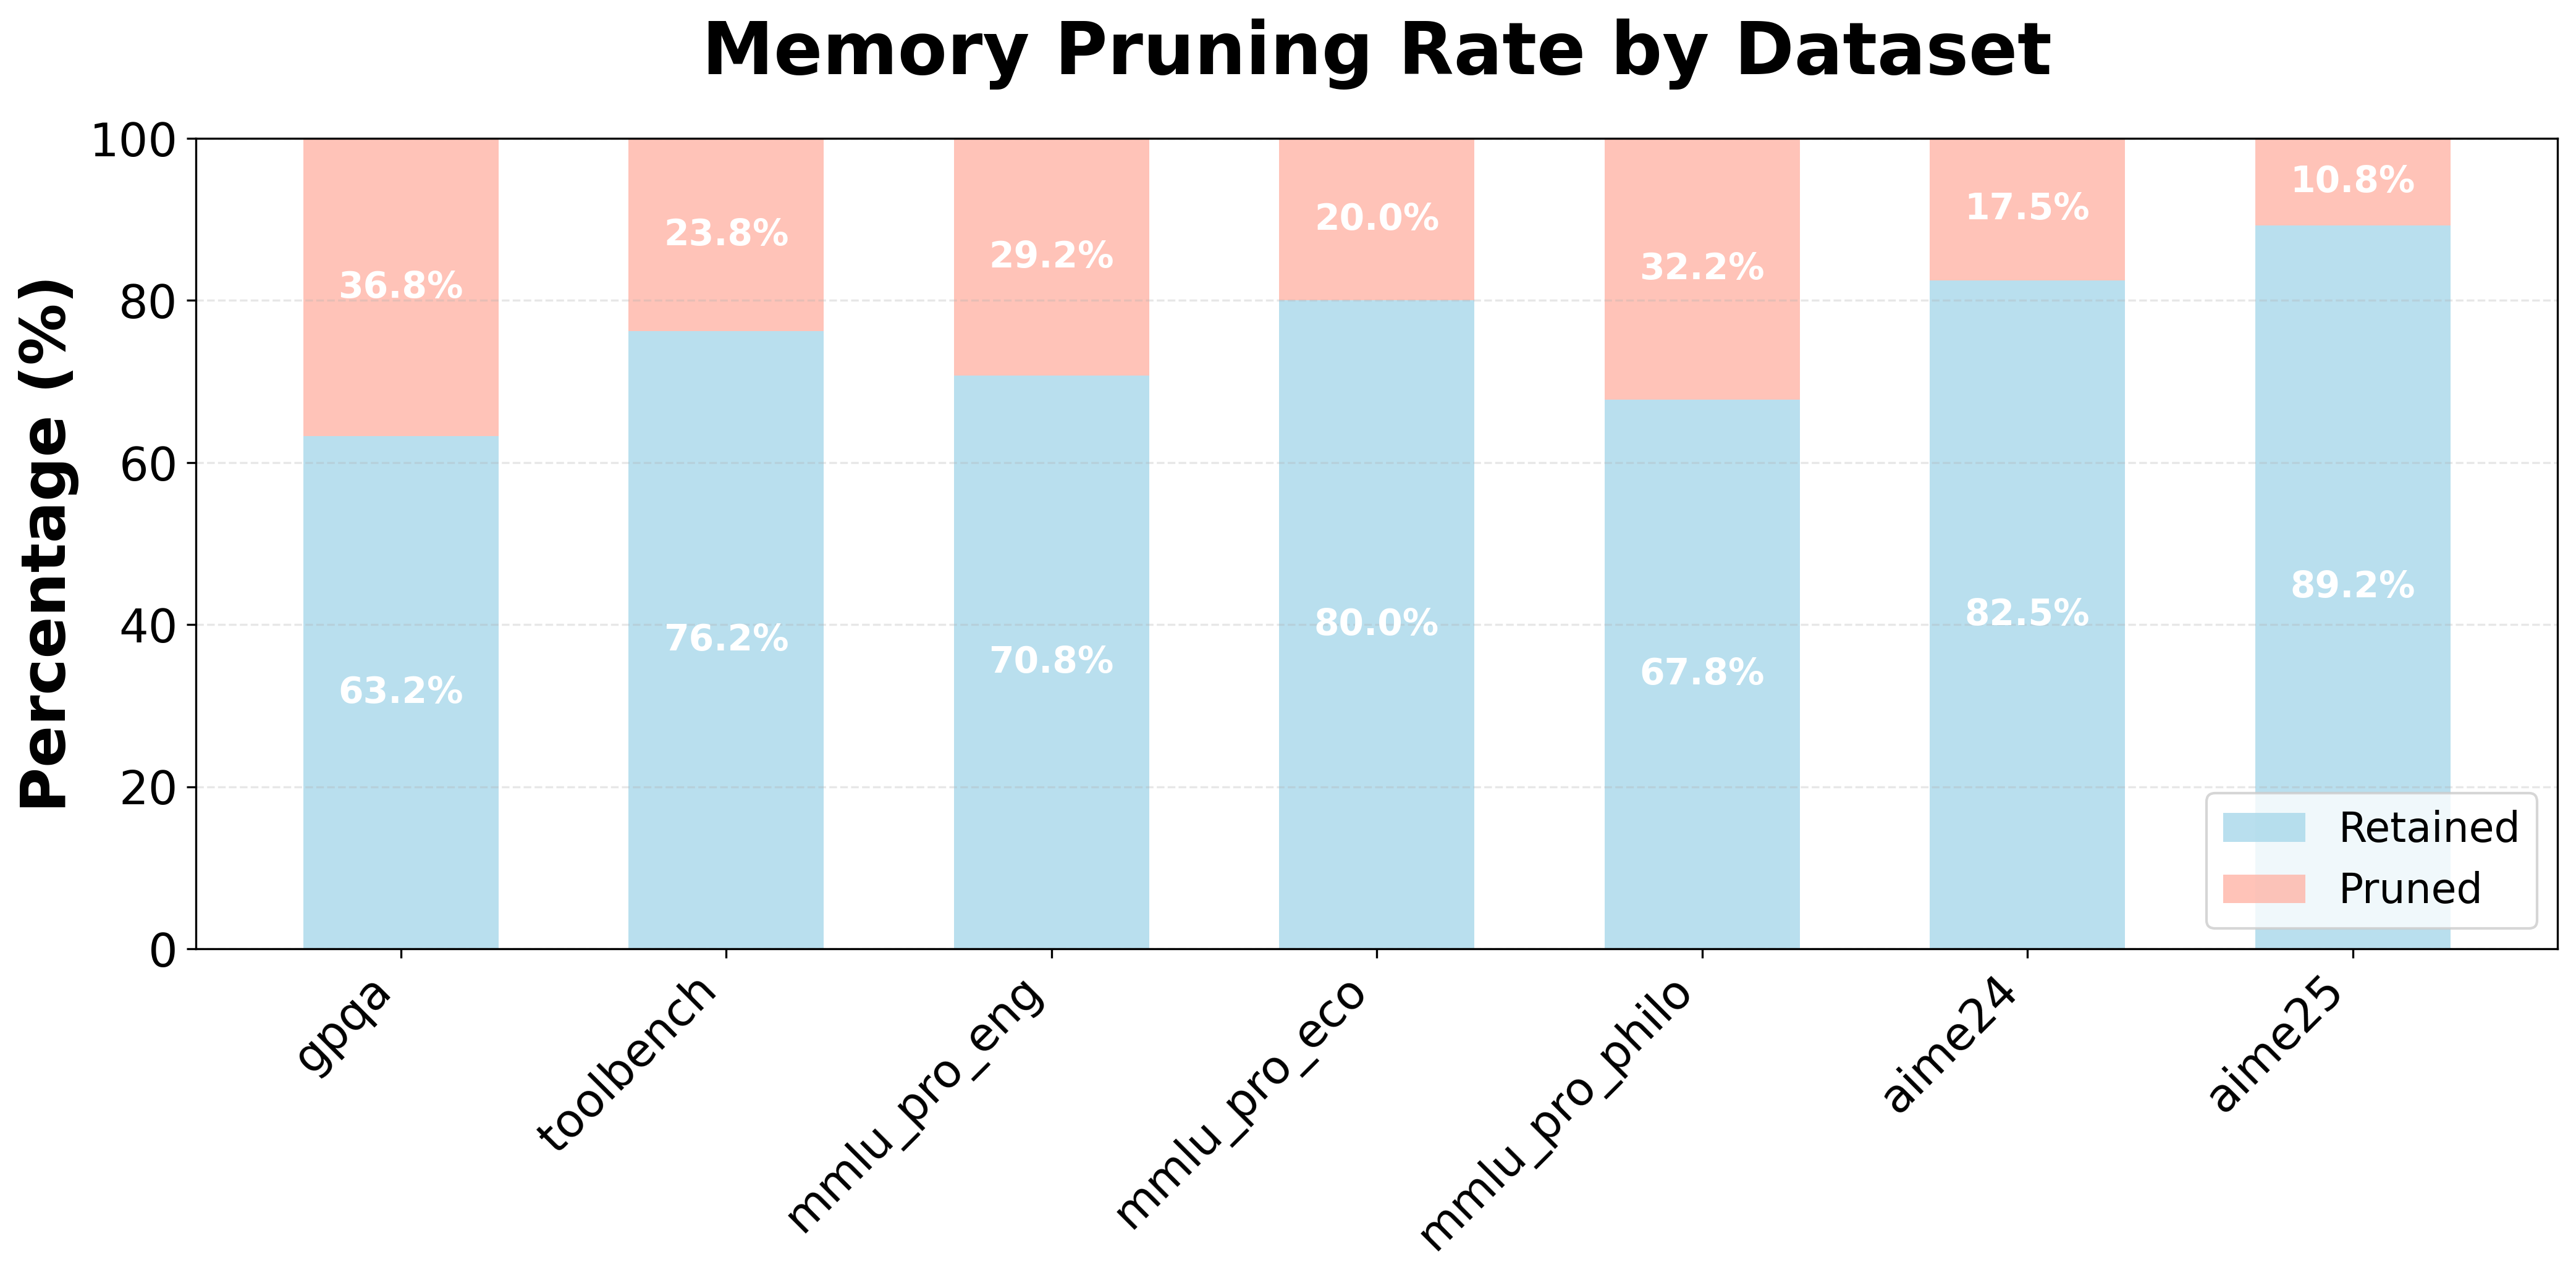
\includegraphics[width=0.95\linewidth]{figures/memory_pruning_analysis.png}
    \caption{Memory pruning rates by dataset. Retained (blue) and pruned (coral) 
memory proportions show varying selectivity across benchmarks.}
    \label{fig:prune}
\end{figure}
\subsection{Additional Analysis of Memory Pruning}
\label{app:memory_prune}
Figure~\ref{fig:prune} shows memory pruning rates across datasets, revealing varying selectivity in memory retention. The pruning ratios differ substantially across benchmarks, which appears related to task diversity and domain coverage. Datasets with broader domain coverage such as GPQA, which encompasses diverse problem types across engineering, physics, and other domains, exhibit higher pruning rates (36.8\%), suggesting that more memories are deemed redundant across heterogeneous tasks. In contrast, datasets with more concentrated problem types like AIME show lower pruning rates (17.5\% and 10.8\% respectively), indicating that memories remain more relevant due to higher task similarity. This pattern suggests that the pruning mechanism effectively identifies and discards domain-irrelevant experiences, though the precise relationship between task diversity and memory selectivity warrants further investigation.








\subsection{Additional Comparative Curves on Single-turn Tasks}
\label{app:curve}
Figure~\ref{fig:compare_single} presents cumulative accuracy curves comparing \alg with the baseline across single-turn reasoning benchmarks and model variants.
As task instances accumulate, \alg shows consistent improvement on GPQA, ToolBench, and MMLU-PRO (Engineer) for both Gemini-2.5-Flash-Lite and Claude-3.7-Sonnet.
Similar to the multi-turn results, History performs comparably at the beginning due to the cold-start phase, but \alg quickly surpasses it as more tasks are processed, indicating the cumulative advantage of continual task-level adaptation.




\begin{figure}[t!]
    \centering
    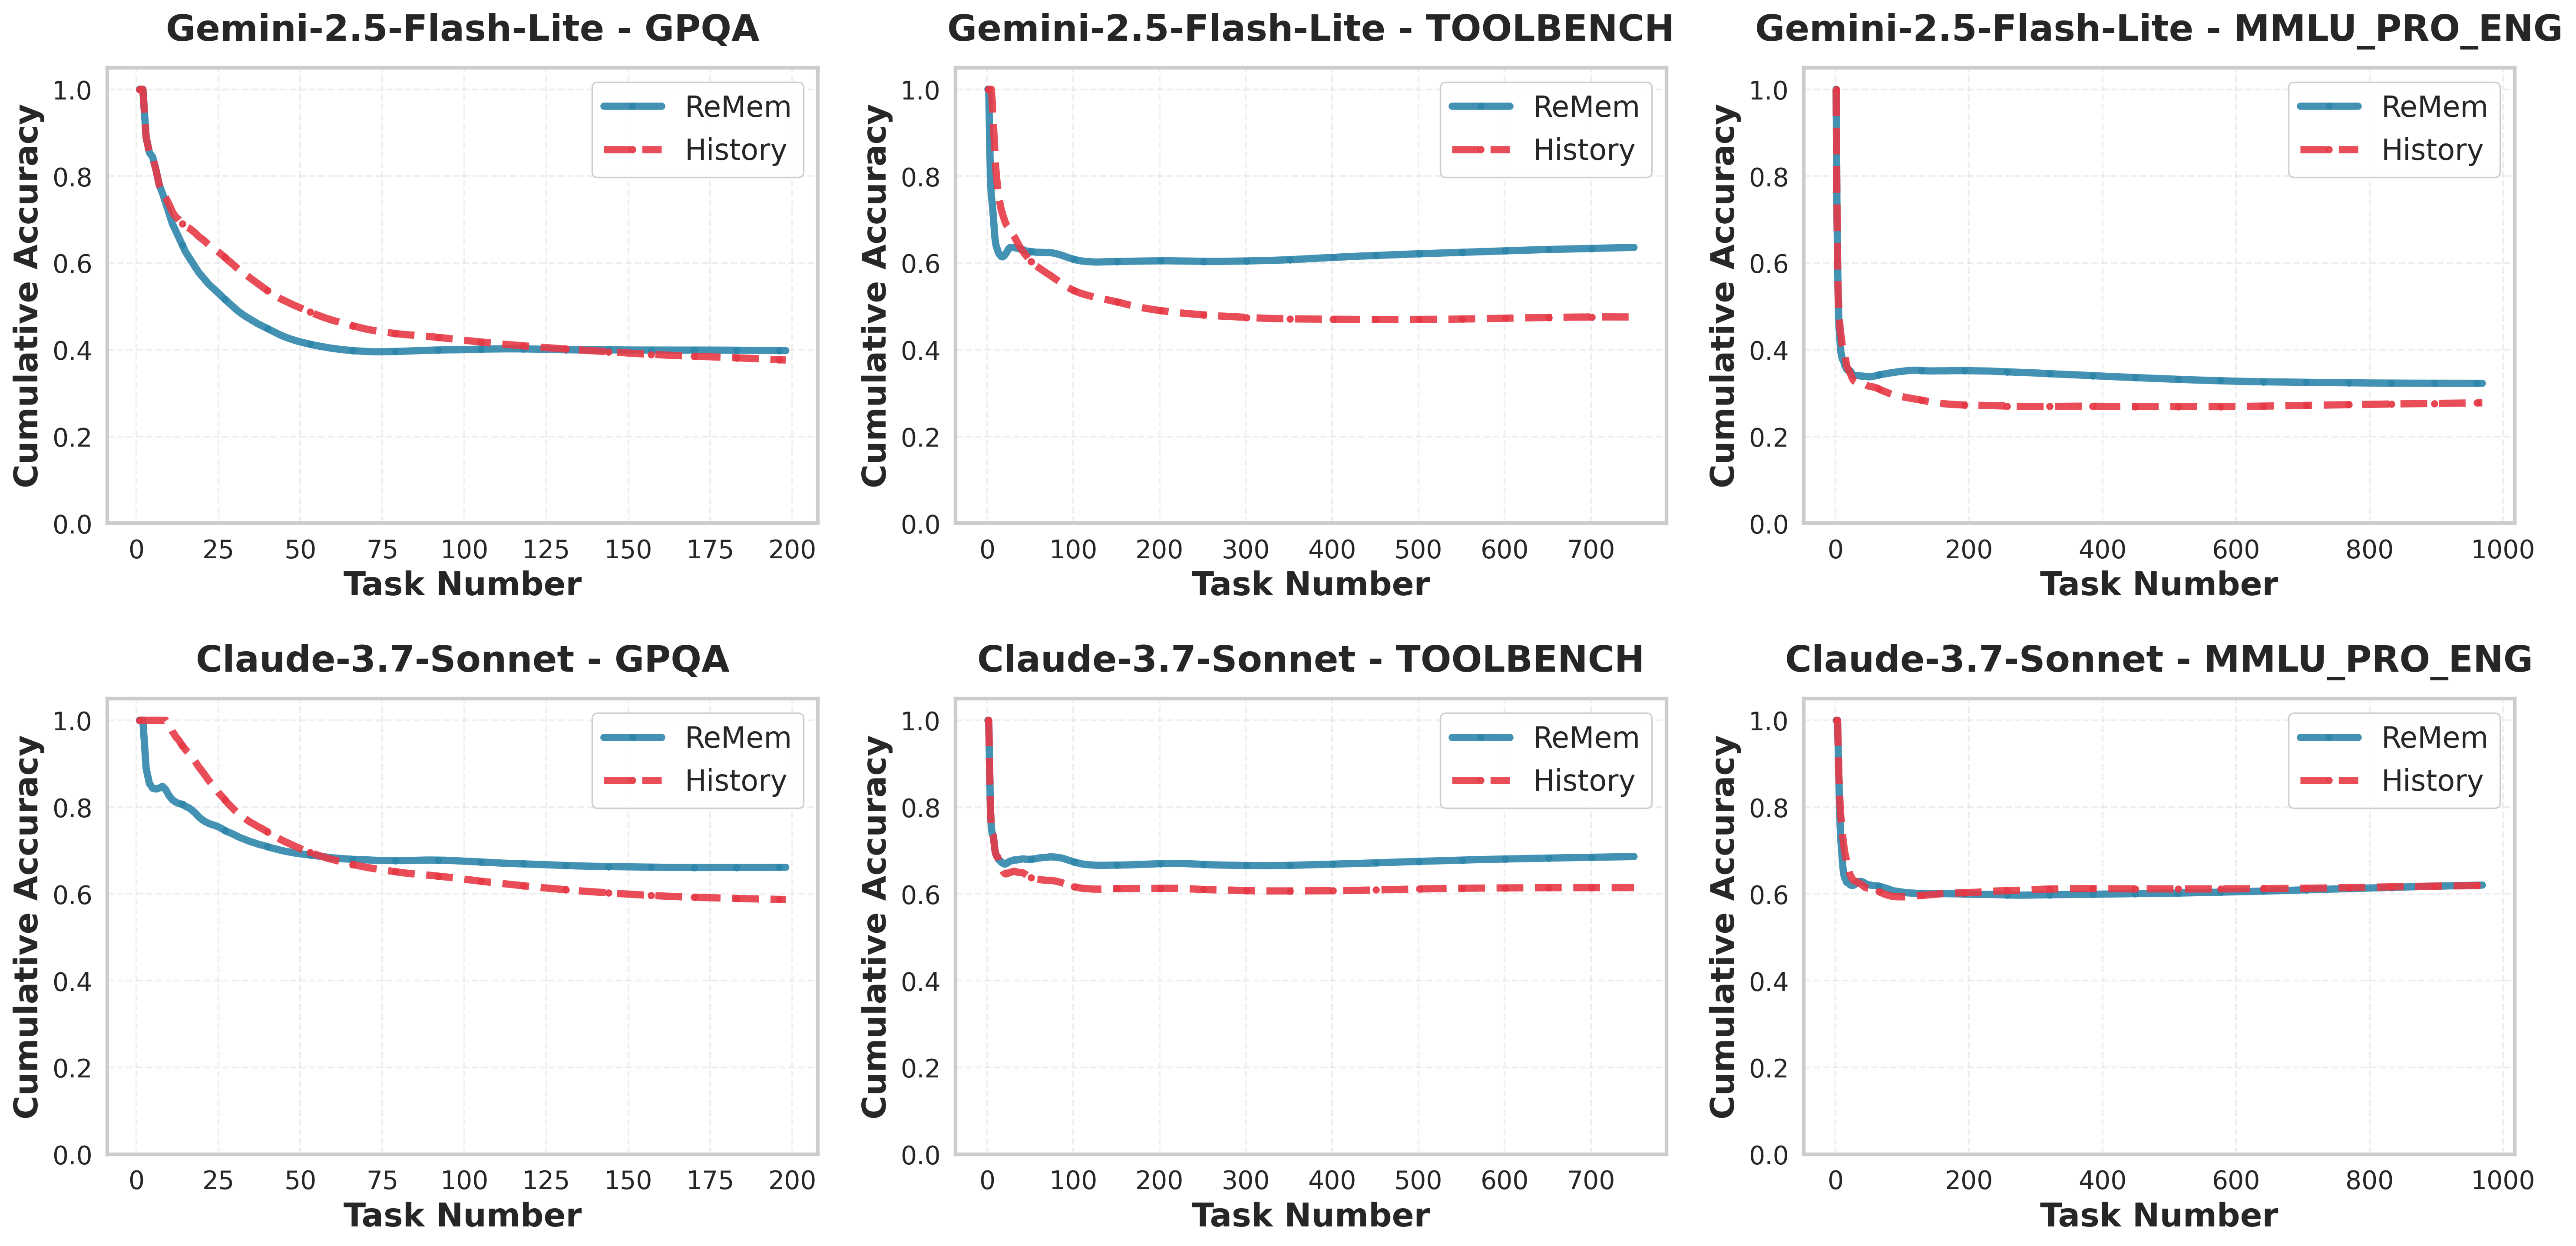
\includegraphics[width=0.95\linewidth]{figures/model_comparison_2x3.png}
    \caption{Cumulative accuracy comparison across model variants and benchmarks. 
ReMem (solid blue) demonstrates consistent improvements over the History baseline 
(dashed red) across Gemini-2.5-Flash-Lite and Claude-3.7-Sonnet models on GPQA, 
TOOLBENCH, and MMLU\_PRO\_ENG datasets. The curves show learning trends as task 
instances accumulate, with ReMem achieving faster convergence and higher final accuracy.}
    \label{fig:compare_single}
\end{figure}
\section{Prompts}


\begin{prompt}{Memory Prompt Template for Multi-turn Dataset}
\small
\textbf{ ==================================================}

\textbf{ENVIRONMENT INSTRUCTIONS}

\textbf{==================================================}

\textit{[Detailed task environment description and rules]}

\textit{Example: Go to kitchen, pick up apple, put it in bag, etc.}

\vspace{12pt}
\textbf{==================================================}

\textbf{EXAMPLE DEMONSTRATIONS}

\textbf{==================================================}

\textit{[Static few-shot examples]}

\textit{Example 1: Goal: ... | Action: ... | Observation: ...}

\textit{Example 2: Goal: ... | Action: ... | Observation: ...}

\vspace{12pt}
\textbf{==================================================}

\textbf{RELEVANT EXPERIENCE FROM SIMILAR TASKS}

\textbf{==================================================}

\textit{[Experience \#1]}

\textit{Goal: [similar goal]}

\textit{Trajectory: [action sequence]}

\textit{Correctness: [success/failure]}

\vspace{6pt}
\textit{[Experience \#2, \#3, ...]}

\vspace{12pt}
\textbf{==================================================}

\textbf{YOUR CURRENT TASK}

\textbf{==================================================}

\textbf{Goal:} \textit{[specific task goal]}

\textit{Help: type 'check valid actions' if action fails}

\textit{Help: type 'inventory' to check items}

\vspace{12pt}
\textbf{==================================================}

\textbf{RECENT HISTORY}

\textbf{==================================================}

\texttt{Observation: [initial environment state]}

\texttt{Action: [previous action]}

\texttt{Observation: [result of previous action]}

\texttt{Action: [previous action]}

\texttt{Observation: [current state]}

\vspace{12pt}
\textbf{==================================================}

\textbf{OUTPUT FORMAT}

\textbf{==================================================}

You MUST respond in EXACTLY ONE of these formats:

\vspace{8pt}
\textbf{Format 1 - Prune experiences:}

\texttt{Think-Prune: <IDs>}

Remove unhelpful experiences from 'RELEVANT EXPERIENCE' section (e.g., ``1,3'' or ``2-4'')

\vspace{8pt}
\textbf{Format 2 - Internal reasoning:}

\texttt{Think: <your reasoning>}

Free-form explanation of your next step

\vspace{8pt}
\textbf{Format 3 - Execute action:}

\texttt{Action: <exact command>}

Must be valid command from ENVIRONMENT INSTRUCTIONS with exact names from RECENT HISTORY


\end{prompt}



\begin{prompt}{Memory Prompt Template for Single-turn Dataset}
You are a helpful assistant with access to LOCAL EXPERIENCE MEMORY. Each memory may contain past experience, rationales, domains, and skills. Below are some retrieved LOCAL EXPERIENCE MEMORIES:

\vspace{6pt}
\textit{[Retrieved/synthesized memories]}

\vspace{6pt}
Now solve the following problem.

\textbf{Question:} \textit{[Your question here]}

\vspace{6pt}
\noindent\textbf{Provide your output in the following format:}
\begin{itemize}
  \item \textbf{Rationale:} your short reasoning, may cite memory if useful
  \item \textbf{Final Answer:} your final answer
\end{itemize}
\end{prompt}


\section{Limitations}
While \method offers a comprehensive evaluation of self-evolving memory, several practical constraints remain. 
Due to budget and API limits, we focus on a selected set of strong LLMs rather than exhaustively covering all available models. 
Additional evaluations on open-weight or multilingual models could further validate the generality of our findings. 
Moreover, our benchmark primarily emphasizes textual and goal-oriented tasks; extending it to richer multimodal or real-world environments would provide a more complete picture of continual memory evolution. 
Despite these limitations, the current study already spans diverse domains, tasks, and architectures, offering a solid foundation for future extensions.


\section{Use of Large Language Models}
During the preparation of this paper, we made limited and controlled use of large language models (LLMs), specifically ChatGPT, as an auxiliary writing aid. 
The LLM was used only for stylistic refinement, including improvements in clarity, grammar, and readability of text originally drafted by the authors. 
All scientific ideas, analyses, experiments, and conclusions were fully developed, written, and verified by the authors. 
Thus, LLMs were employed solely as a language-editing tool, without contributing to the intellectual or scientific content of the work.

